\section{Evaluation}
\label{sec:eval}

We have implemented our approach in \toolname: a system for repairing parse
errors for \python at its entirety. Next, we describe our implementation and an
evaluation that addresses four questions:

\begin{itemize}
    \item \textbf{RQ1}: How \emph{accurate} are \toolname's predicted error production rules?
                        (\S~\ref{sec:eval:accuracy})
    \item \textbf{RQ2}: How \emph{precisely} can \toolname repair parse errors?
                        (\S~\ref{sec:eval:precise})
    \item \textbf{RQ3}: How \emph{efficiently} can \toolname repair parse errors?
                        (\S~\ref{sec:eval:efficiency})
    \item \textbf{RQ4}: How \emph{useful} are \toolname's suggested repairs?
                        (\S~\ref{sec:eval:useful})
\end{itemize}

% \subsection{Implementation} \label{sec:eval:gen_method}

\mypara{Training Dataset}
For our evaluation, we use the \python dataset we used in our error data
analysis in \autoref{sec:error-analysis} gathered from
PythonTutor.com~\citep{Guo2013} between the years 2017 and 2018. The dataset has
more than 1,100,000 usable erroneous Python programs and their respective fixes.
The programs have an average length of \emph{87 tokens}, while the abstracted
token sequences have a much shorter average of \emph{43 tokens}. We choose
15,000 random programs from the dataset for all our tests, and the rest we use
as our training set.

We first learn a PCFG on the training set of fixed programs in order to learn
the probabilities for each production rule in the \emph{full set of the \python
grammar}. \toolname then extracts the abstracted token sequences for all
programs in the training set. Next, while for the full set of \python there are
\emph{455 possible terminal error production rules} that \toolname's can predict
from, in reality only \emph{340 error rules} are ever used in the full dataset.
We arrive at this set of error rules by parsing all the erroneous programs in
the training set with the ECE-Parser and the "diff" error rules, as described in
\autoref{sec:overview:train}. Each program is also assigned as labels these
error rules that make the ECE-Parser parse the erroneous program successfully.

\mypara{Transformer Classifier}
\toolname's error rule prediction uses a Transformer classifier with \emph{six}
transformer blocks, that each has a fully-connected hidden layer of 256 neurons
and 12 attention heads. The output of the transformer blocks is then connected
to a \dnn based classifier with \emph{two} fully-connected hidden layers of 256
and 128 neurons respectively. The neurons use rectified linear units (ReLU) as
their activation function \citep{Nair2010-xg}, while the output layer uses the
sigmoid function for each class \citep{Nielsen2015-pu}. Additionally, the are
\emph{two input embedding layers} of a length of 128, one for input tokens and
one for their positions in the sequence. We also limit the size of the input
abstracted token sequences to a length of 128, which covers $95.7\%$ of the
training set, without the need of pruning them. Finally, the Transformer
classifier was trained using an \textsc{Adam} optimizer \citep{Kingma2014-ng}, a
variant of stochastic gradient descent that converges faster, for a total of 50
epochs.

\subsection{RQ1: Accuracy}
\label{sec:eval:accuracy}

We consider \toolname's transformer classifiers' accuracy up to the \emph{top
50} error production rules predictions against our original and the final
version of our approach

% colors from http://colorbrewer2.org/?type=sequential&scheme=Blues&n=3
\definecolor{blue1}{HTML}{DEEBF7}
\definecolor{blue2}{HTML}{9ECAE1}
\definecolor{blue3}{HTML}{3182BD}
\definecolor{green1}{HTML}{E5F5E0}
\definecolor{green2}{HTML}{A1D99B}
\definecolor{green3}{HTML}{31A354}

\begin{figure}[t]
  % \begin{minipage}[c]{0.49\linewidth}
    \centering
    \resizebox{0.6\linewidth}{!}{
      \Large
      \begin{tikzpicture}
      \begin{axis}[
        ybar stacked,
        width=1.1\linewidth,
        height=11cm,
        % title={Accuracy of Repair Template Prediction},
        ylabel={Prediction Accuracy (\%)},
        bar width=1cm,
        ymin=0.0,
        ymax=101.0,
        ytick={0.0, 10.0, 20.0, 30.0, 40.0, 50.0, 60.0, 70.0, 80.0, 90.0, 100.0},
        yticklabel={\pgfmathparse{\tick}\pgfmathprintnumber{\pgfmathresult}},
        ytick style={draw=none},
        ymajorgrids = true,
        symbolic x coords={original, abstracted, abstracted-best},
        enlarge x limits=0.3,
        xtick=data,
        xtick style={draw=none},
        xticklabels={\textsc{Original}\xspace, \textsc{Abstracted}\xspace, \textsc{Threshold}\xspace},
        %x tick label style={rotate=45, anchor=north east},
        % x tick label style={font=\small},
        % y tick label style={font=\small},
        reverse legend,
        % transpose legend,
        legend style={legend pos = north east, legend columns=4, font=\small},
      ]

      \addplot[draw=black, fill=blue2, bar shift=-.501cm, postaction= { pattern=dots }] coordinates {(original, 0.0) (abstracted, 0.0) (abstracted-best, 79.28025102961365)};

      \resetstackedplots

      \addplot[draw=black, fill=green2, bar shift=.501cm, postaction= { pattern=dots }] coordinates {(original, 0.0) (abstracted, 0.0) (abstracted-best, 69.82968369829683)};

      \resetstackedplots

      \addplot[draw=black, fill=green1, bar shift=.501cm] coordinates {(original, 12.875536480686696) (abstracted, 58.394160583941606) (abstracted-best, 0.0)};
      \addlegendentry{Top-10}
      \addplot[draw=black, fill=green2, bar shift=.501cm] coordinates {(original, 20.100143061516448) (abstracted, 14.922952149229523) (abstracted-best, 0.0)};
      \addlegendentry{Top-20}
      \addplot[draw=black, fill=green3, bar shift=.501cm] coordinates {(original, 31.974248927038623) (abstracted, 15.49067315490673) (abstracted-best, 0.0)};
      \addlegendentry{Top-50}
      \addlegendimage{empty legend}
      \addlegendentry{Rare:}

      \resetstackedplots

      \addplot[draw=black, fill=blue1, bar shift=-.501cm] coordinates {(original, 56.712132089016514) (abstracted, 72.11217885859972) (abstracted-best, 0.0)};
      \addlegendentry{Top-10}
      \addplot[draw=black, fill=blue2, bar shift=-.501cm] coordinates {(original, 11.769733018835673) (abstracted, 9.335163757599531) (abstracted-best, 0.0)};
      \addlegendentry{Top-20}
      \addplot[draw=black, fill=blue3, bar shift=-.501cm] coordinates {(original, 18.65107852186101) (abstracted, 11.253840622344256) (abstracted-best, 0.0)};
      \addlegendentry{Top-50}
      \addlegendimage{empty legend}
      \addlegendentry{All:}

      \end{axis}
      \end{tikzpicture}
    }
    \caption{
      Results of our error production rule prediction classifiers for the simple original token sequences and their abstracted versions using the PCFG.
    }
    \label{fig:accuracy-results}
  % \end{minipage}
  % \begin{minipage}[c]{0.49\linewidth}
  %   \centering
  %   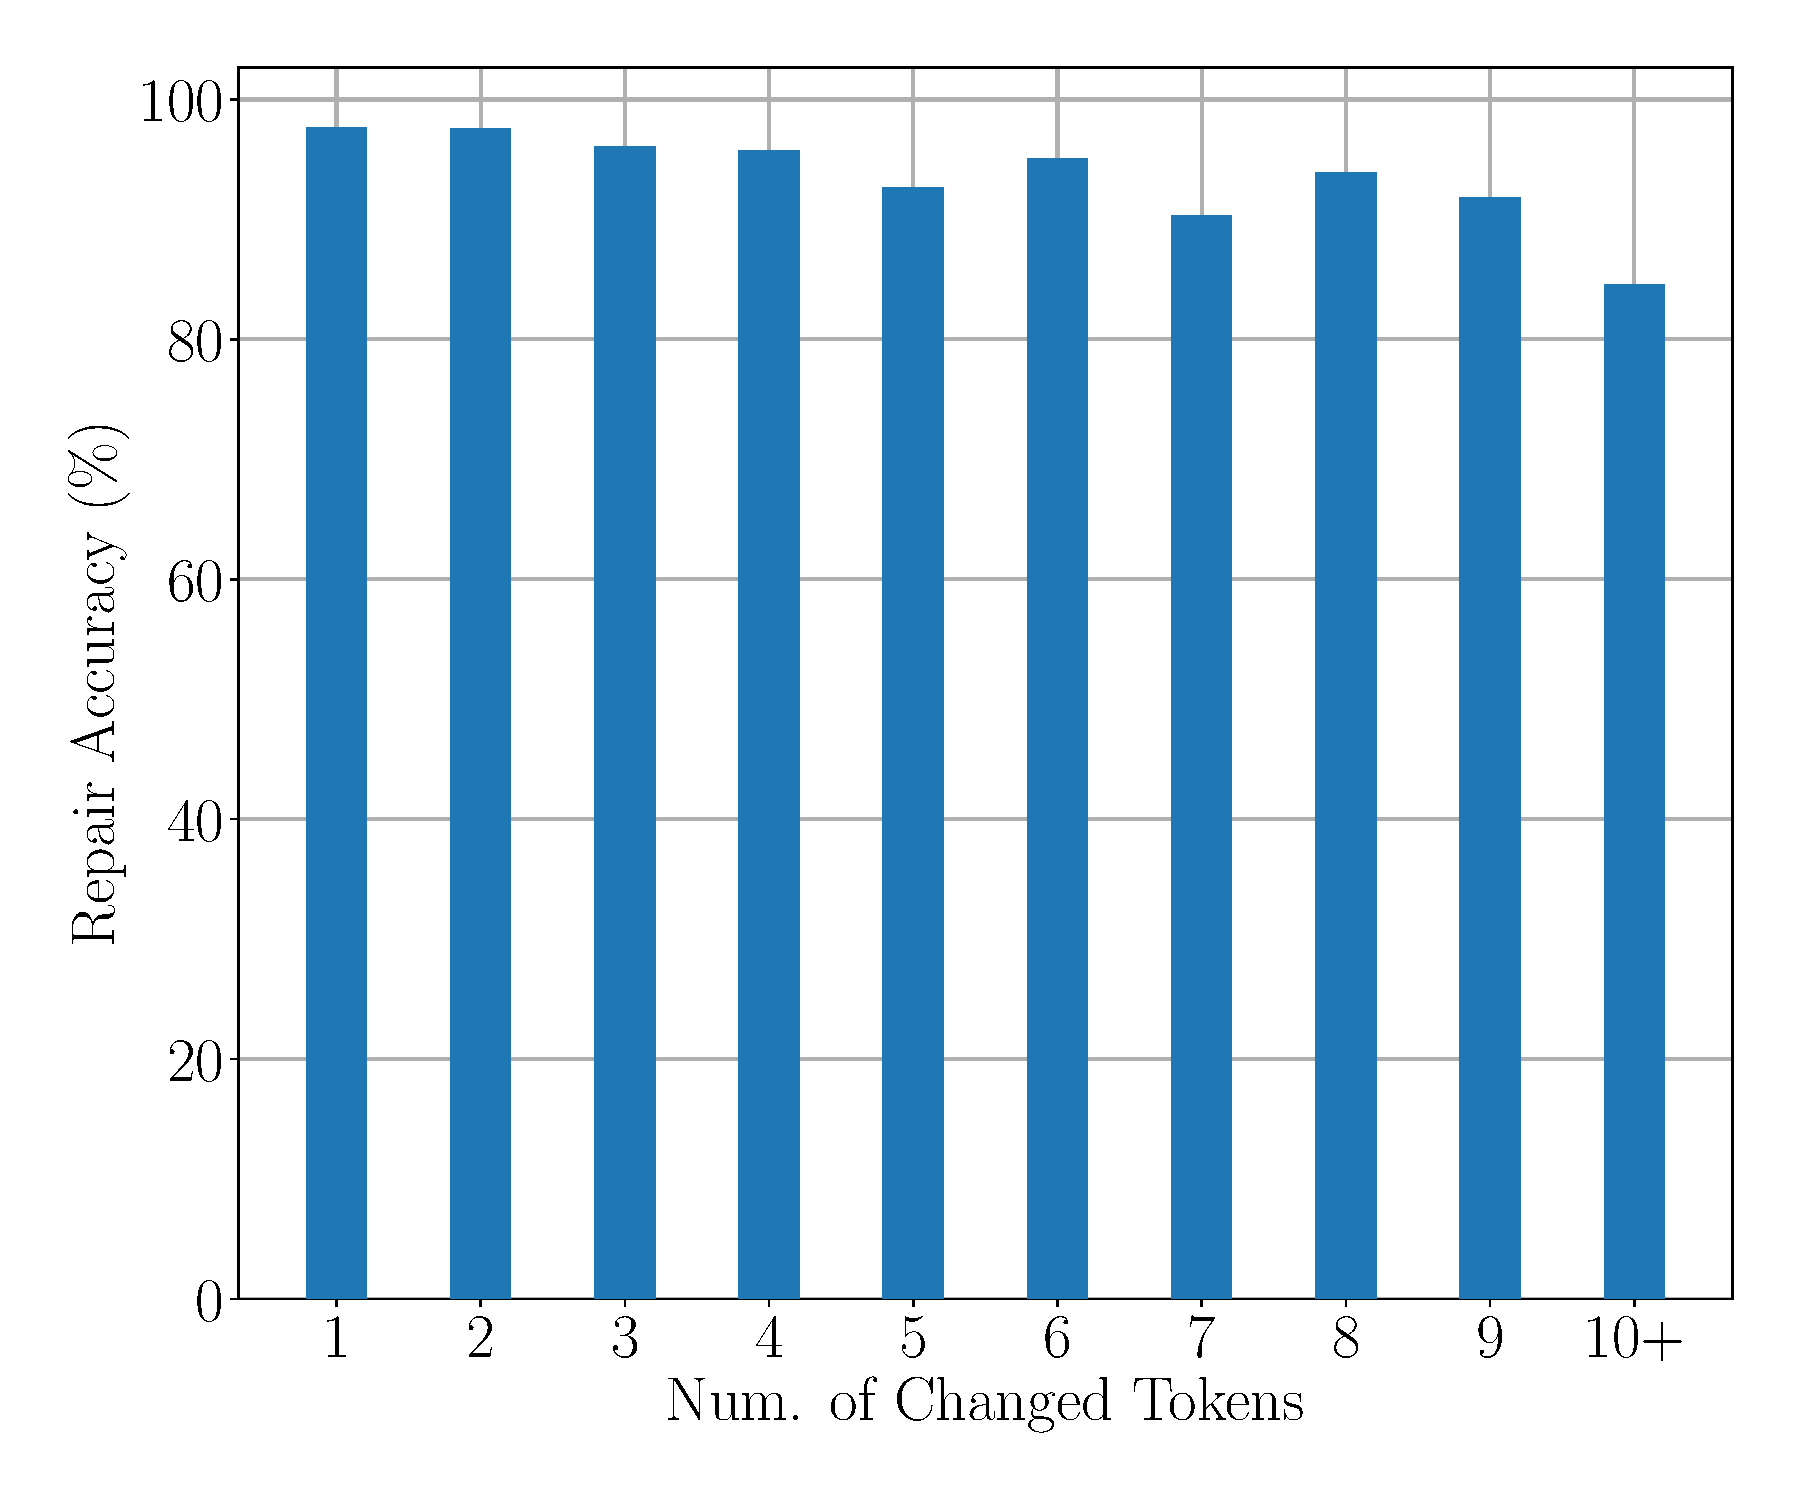
\includegraphics[width=\linewidth]{accuracy-per-change.pdf}
  %   \caption{The repair accuracy for the number of edits needed by the user to repair.}
  %   \label{fig:accuracies-per-changes}
  % \end{minipage}
\end{figure}


% \mypara{Results: Accuracy of Error Rule Prediction}
%
\autoref{fig:accuracy-results} shows the accuracy results of our error
production rule prediction experiments. The y-axis describes the
\emph{prediction accuracy}, \ie the fraction of test programs for which the
correct \emph{full set} of error rules to repair the program was predicted in
the top-K sorted rules.
%
The \textsc{Original} version of our transformer classifier didn't consider the
abstracted token sequences and used the full \textsc{Original} token sequences,
whose results are presented in the first two bars of
\autoref{fig:accuracy-results}. The next two bars show our final results using
the \textsc{Abstracted} token sequences to train the classifier. Finally, the
last two dotted bars show the results for when a \textsc{Threshold} is set in
order to select the predicted error rules, instead of picking the static top-K
ones. The predicted error rule set can have a size anywhere between 1 and a
maximum of 25 (pre-defined by us based on the top-K results).

The blue bars show the accuracy on the full test set of \textsc{All} 15,000 test
programs, while the green bars show the results on the subset of the
\textsc{Rare} programs, \ie the programs that didn't include any of the 50 most
popular error rules, that amount only for 4.8\% of our test set.

The \textsc{Original} predictor, even with the Top-50 predicted error rules is
less accurate than the Top-20 predictions of the \textsc{Abstracted}, with an
accuracy of 87.13\%, which drops to 68.48\% and 56.71\% respectively for the
Top-20 and Top-10 predictions. The \textsc{Abstracted} predictor significantly
outperforms the \textsc{Original} predictor with a 72.11\% Top-10 accuracy,
81.45\% Top-20 accuracy and 92.70\% Top-50 accuracy.

The \textsc{Threshold} predictions are almost as accurate as the
\textsc{Abstracted} Top-20 predictions with an accuracy of 79.14\% and a median
number of selected error rules of 11 (average 13.2). This could potentially mean
that this predictor is a valid alternative for the static Top-20 predictions.

Finally, we observe that our \textsc{Abstracted} classifiers generalize
efficiently for our dataset of erroneous \python programs and is almost as
accurate for the \textsc{Rare} programs as the rest of the dataset with a
73.32\% Top-20 accuracy (88.81\% Top-50 accuracy). The same holds for the
\textsc{Threshold} predictions with a 66.42\% accuracy.

\begin{framed}
  \noindent \toolname's transformer classifier learns to encode programs with
  syntax errors and select candidate error production rules for them
  effectively, yielding \emph{high accuracies}. By abstracting the tokens
  sequences, \toolname is able to \emph{generalize} better and make more
  accurate predictions with a \emph{81.45\% Top-20 accuracy}.
\end{framed}


\subsection{RQ2: Repaired Program Preciseness}
\label{sec:eval:precise}

Next we evaluate \toolname's end-to-end accuracy and preciseness in generating
valid parses for programs with syntax errors. For all of our tests we limit
\toolname's parsing time to \emph{5 mins} and run our experiments on the 15,000
program  test set. Additionally, we use here the highest-performing transformer
classifier, the \textsc{Abstracted} classifier.

We compare \emph{two versions} of our implementation of \toolname
(\textsc{AllParses} and \textsc{MinimumCost}) against two versions of the
error-correcting parser with a static selection of the 20 and 50 most popular
error production rules in our training set. We make this comparison because we
observe in our training set that the 50 most of popular error rules are used for
parsing as much as \emph{86\%} of the dataset.

Our \textsc{AllParses} ECE-Parser and \textsc{MinimumCost} ECE-Parser both use
the \emph{Top-20 predictions} from our \textsc{Abstracted} classifier to parse
and repair buggy programs. The \textsc{AllParses} ECE-Parser keeps internally
\emph{all possible states} that arise from using the predicted error rules
similarly to the original ECE-Parser described in \citep{Aho_1972}. We use a
maximum repair cost of 2 edits (\ie a maximum of 2 insertions, deletions or
replacements) to limit the search space. The \textsc{MinimumCost} version
however keeps always the minimum-edit repair and discards all other states that
may lead to a higher cost. This allows for a higher maximum cost of 10 edits.
Finally, while \textsc{AllParses} can generate a large number of repairs, we
keep only the top 3 repairs after filtering with a static code checker
(\textsc{Pylint}, \url{https://www.pylint.org/}) as most developers will
consider at most five suggestions before falling back to manual debugging
\citep{Kochhar2016-oc, Parnin2011-ce}.

\autoref{tab:seq2parse_full_results} shows the percentage of test programs that
each of these four versions can parse successfully (\ie the parse accuracy), the
rare programs parse accuracy and the amount of parses that match the one that
user compiled. We observe that the Top-20 predictions with the
\textsc{MinimumCost} ECE-Parser \emph{outperforms} every other option with
94.25\% parse accuracy and 94.01\% rare parse accuracy. It also achieves to
generate the intended user parse for 20.55\% of the set, \ie over 1 out 5 of the
cases. The 20 most popular ECE-Parser with 79.81\% parse accuracy and 65.01\%
rare parse accuracy is much less accurate, and achieves 4.24\% less times to
generate the user parse, while the 50 most popular is slightly less accurate
with 90.03\% and 79.82\% accuracy. The 50 most popular ECE-Parser has also a
high user fix accuracy of 18.55\%. The \textsc{AllParses} ECE-Parser has a lower
parse accuracy of 59.31\% in general, however it manages to generate the user
fix 30.57\% of the times and achieve a 71.47\% rare accuracy. It thus achieves
to parse almost one out of three programs with syntax errors, while being able
to parse even the rare programs.

\begin{framed}
  \noindent \toolname can \emph{parse and repair 94.25\%} of programs with
  syntax errors, while also generating \emph{the user fix over 1 out 5 of
  cases}.
\end{framed}

% \begin{table}[t]
%   \centering
%   \begin{tabular}{l||cccc}
%     Error Rule Approach            & Parse Accuracy & User Parse Rate & Parse time & Speedup \\
%     \hline
%     20 Most Popular                & 79.81\% & 16.31\% & 4.8 sec  & 45.8 sec \\
%     50 Most Popular                & 90.03\% & 18.55\% & 10.6 sec & 37.1 sec \\
%     Top-20 (\textsc{AllParses})   & 59.31\% & 30.57\% & 15.6 sec & 57.4 sec \\
%     Top-20 (\textsc{MinimumCost}) & 92.45\% & 19.95\% & 5.3 sec  & 68.0 sec \\
%   \end{tabular}
%   \caption{Experimental results of \toolname's repair approaches.}
%   \label{tab:seq2parse_full_results}
% \end{table}

\begin{figure}[t]
  \centering
  \begin{minipage}[c]{0.46\linewidth}
    \centering
    \resizebox{\linewidth}{!}{
      \begin{tabular}{l||ccc}
        Error Rule            & Parse            & Rare Parse       & User Fix \\
        Approach              & Accuracy         & Accuracy         & Accuracy \\
        \hline
        20 Most Popular       & 79.81\%          & 65.01\%          & 16.31\% \\
        50 Most Popular       & 90.03\%          & 79.82\%          & 18.55\% \\
        \textsc{AllParses}    & 59.31\%          & 71.47\%          & \textbf{30.57\%} \\
        \textsc{MinimumCost}  & \textbf{94.25\%} & \textbf{94.01\%} & 20.55\% \\
      \end{tabular}
    }
    \caption{Experimental results of \toolname's repair approaches.}
    \label{tab:seq2parse_full_results}
  \end{minipage}
  \begin{minipage}[c]{0.53\linewidth}
    \centering
    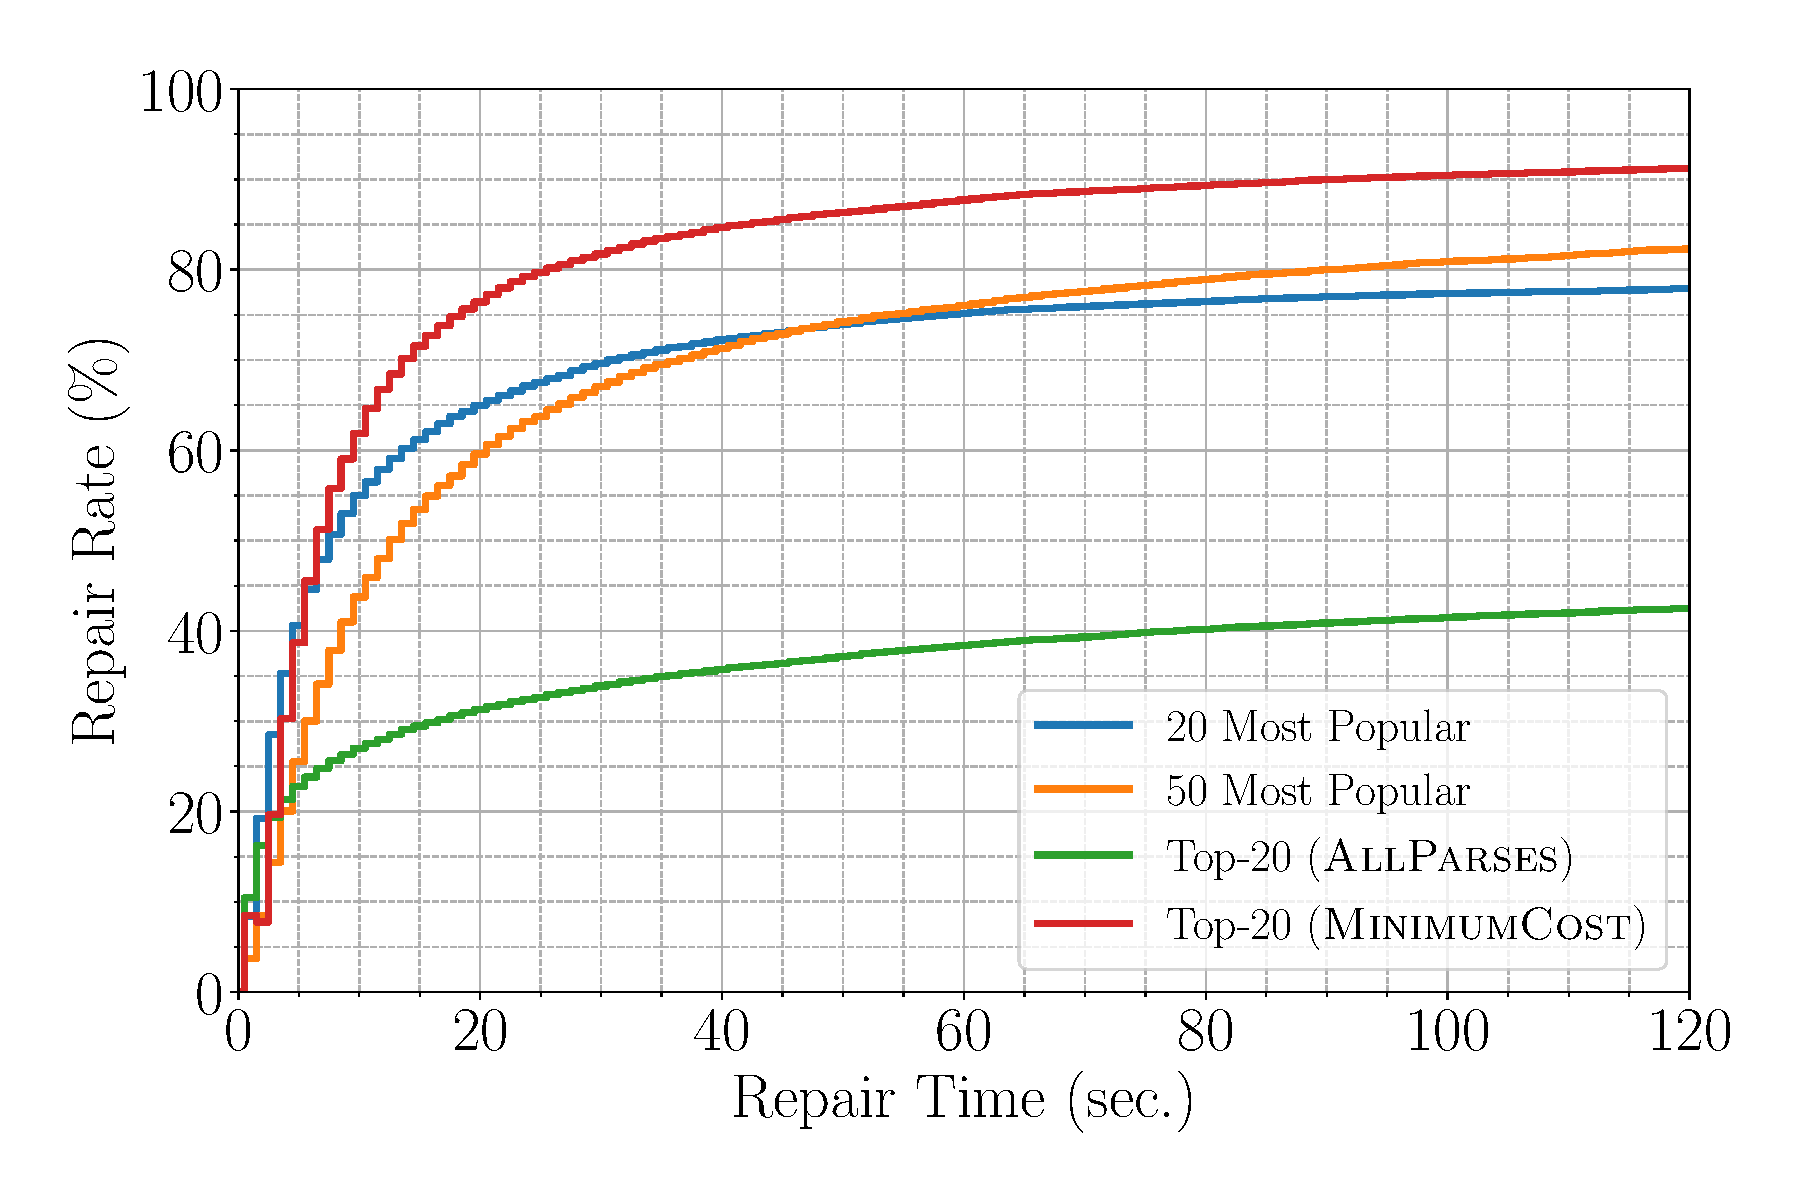
\includegraphics[width=\linewidth]{tool-repair-rate.pdf}
    \caption{The repair rate for all the approaches in
    \autoref{tab:seq2parse_full_results}}
    \label{fig:tool-repair-rate}
  \end{minipage}
\end{figure}

\subsection{RQ3: Efficiency}
\label{sec:eval:efficiency}

% \begin{figure}[t]
%   \centering
%   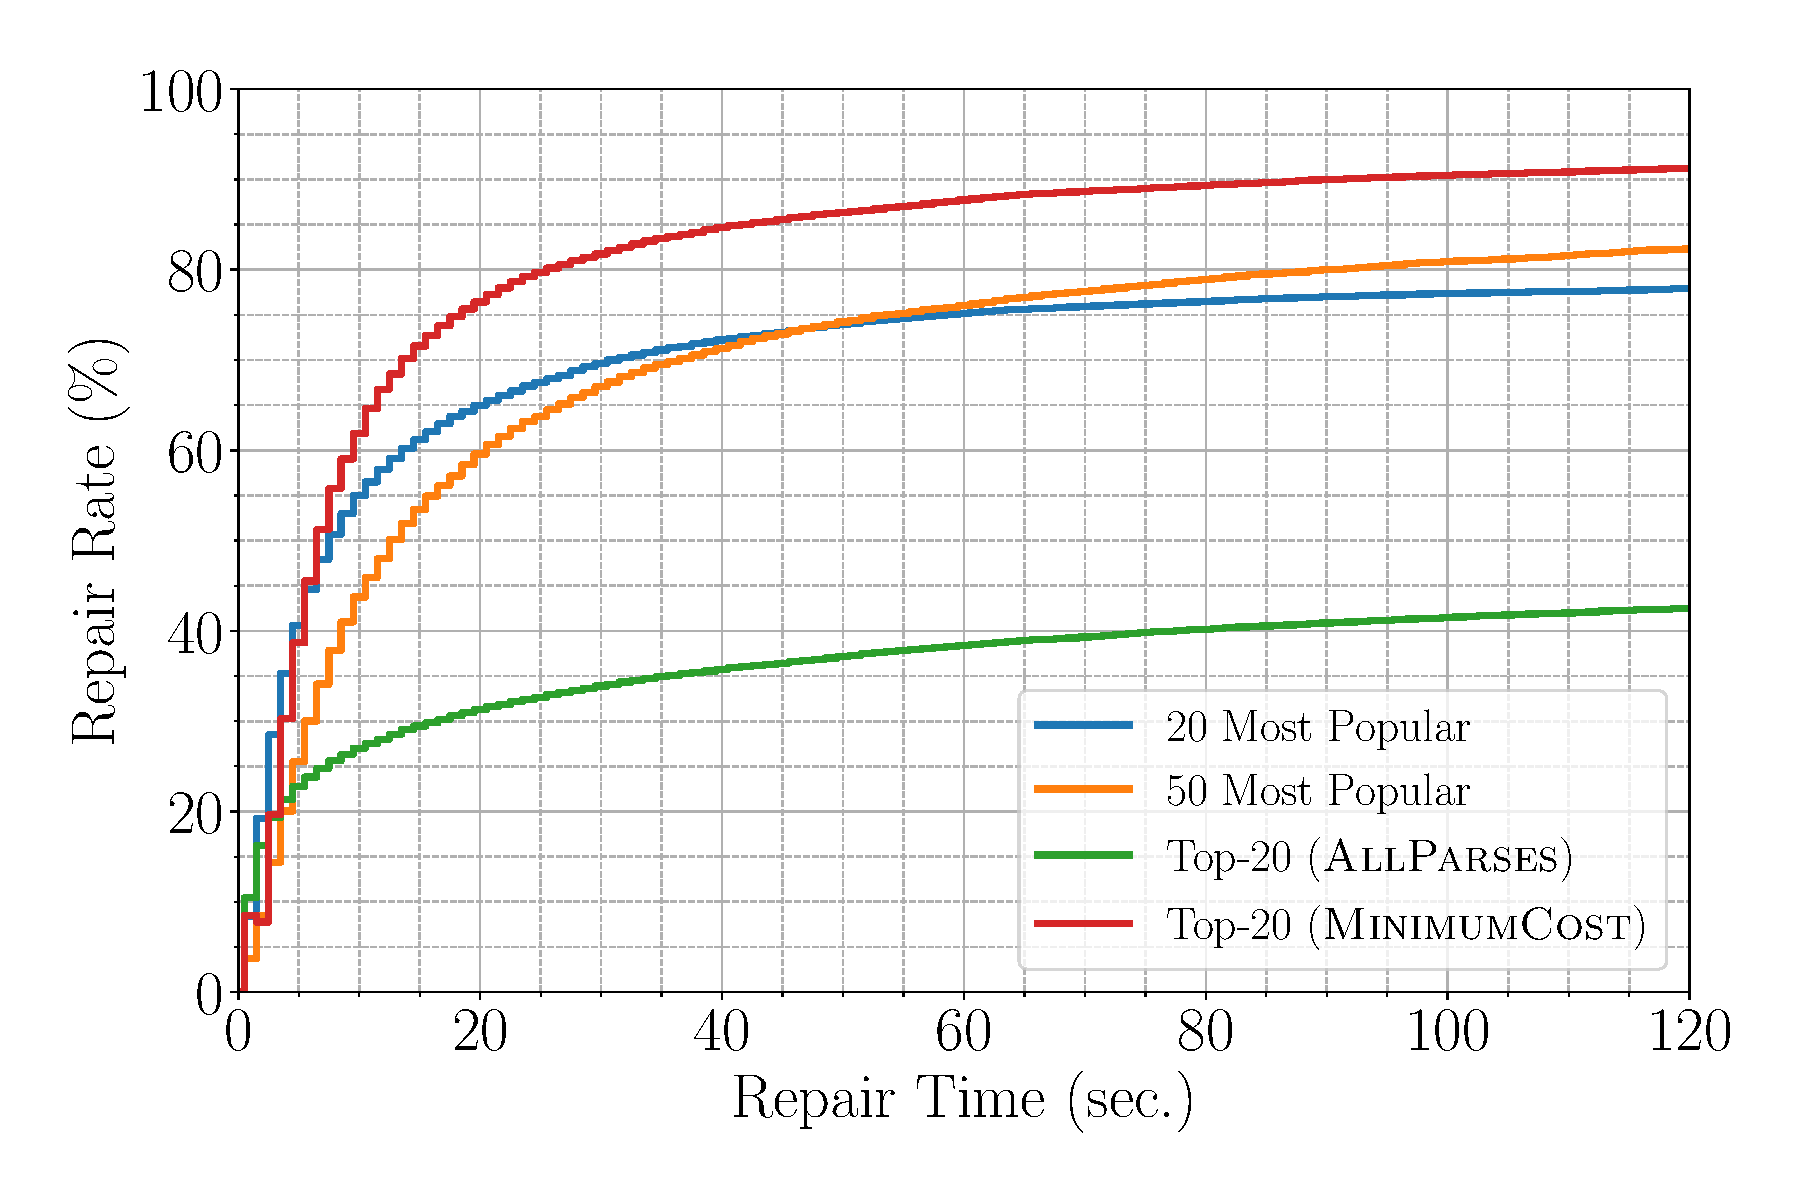
\includegraphics[width=0.8\linewidth]{tool-repair-rate.pdf}
%   \caption{The repair rate for all the approaches in
%   \autoref{tab:seq2parse_full_results}}
%   \label{fig:tool-repair-rate}
% \end{figure}

Next we evaluate \toolname's efficiency by measuring how many programs it is
able to parse. We limit each ECE-Parser to 5 minutes. (In general the procedure
is undecidable, and we conjecture that a longer timeout will diminish the
practical usability for novices.) We compare the efficiency of \toolname for all
the versions of \autoref{tab:seq2parse_full_results}.

\autoref{fig:tool-repair-rate} shows the cumulative distribution function of all
\toolname approaches' repair rates over their parse time. We observe that using
the top 20 error production rule predictions is the most efficient while
maintaining the highest parse accuracy at all times, with a repair rate of
82.1\% within 30 seconds and a median parse time of 5.3 seconds.

We observe that, using a fixed set of the 20 and 50 most popular rules for
\toolname to parse programs with syntax errors, a 70.0\% and 67.56\%
respectively within 30 seconds, and median parse times of 4.8 and 10.6 seconds
respectively. The 50 most popular ECE-Parser is parses less programs until the
45 seconds but the extra number of error rules aids the ECE-Parser to parse more
after that point and outperform the 20 most popular ECE-Parser.

We also observe that \toolname successfully parses around 34.1\% of the programs
with its \textsc{AllParses} approach in 30 seconds and has a median parse time
of 15.6 seconds. While this approach is much less efficient that the others. due
to the vast amount of states is keeps internally in its data structure, it is
also able to generate the exact human repair in 1 out of 3 times which makes
still a very valuable approach (\S~\ref{sec:eval:precise}).

\begin{framed}
  \noindent \toolname can parse programs with syntax errors for the vast
  majority of the test set in under 30 seconds.
\end{framed}

\subsection{RQ4: Usefulness}
\label{sec:eval:useful}
